Naast de CPU is er ook een GPU\index{GPU}, ofwel Graphical Processing Unit\index{Graphical Processing Unit}. De GPU zorgt voor de aansturing van het beeldscherm. Vooral voor gaming zijn er vaak zware processoren nodig om alle 3D beelden te renderen. Moderne grafische kaarten\index{Grafische kaart}\index{Graphical card} zijn bijna zelfstandige computers. Ze hebben hun eigen processor en hun eigen geheugen (VRAM\index{VRAM}\index{Video RAM}).

Waar de CPU goed is in het behandelen van \'e\'en grote taak en er daarvan meerdere achter elkaar (serieel) kan behandelen, met enkele parallel, is de GPU beter in het behandelen van kleine opdrachten parallel. Een CPU heeft dan ook vaak enkele cores, terwijl een GPU enkele duizenden cores kan hebben.

Zowel een CPU als een GPU heeft koeling nodig om de warmte die wordt geproduceerd af te voeren. Een voorbeeld is een RTX 380 zoals weergegevn in \ref{fig:gpu:ventilator}.

\begin{figure}[h]
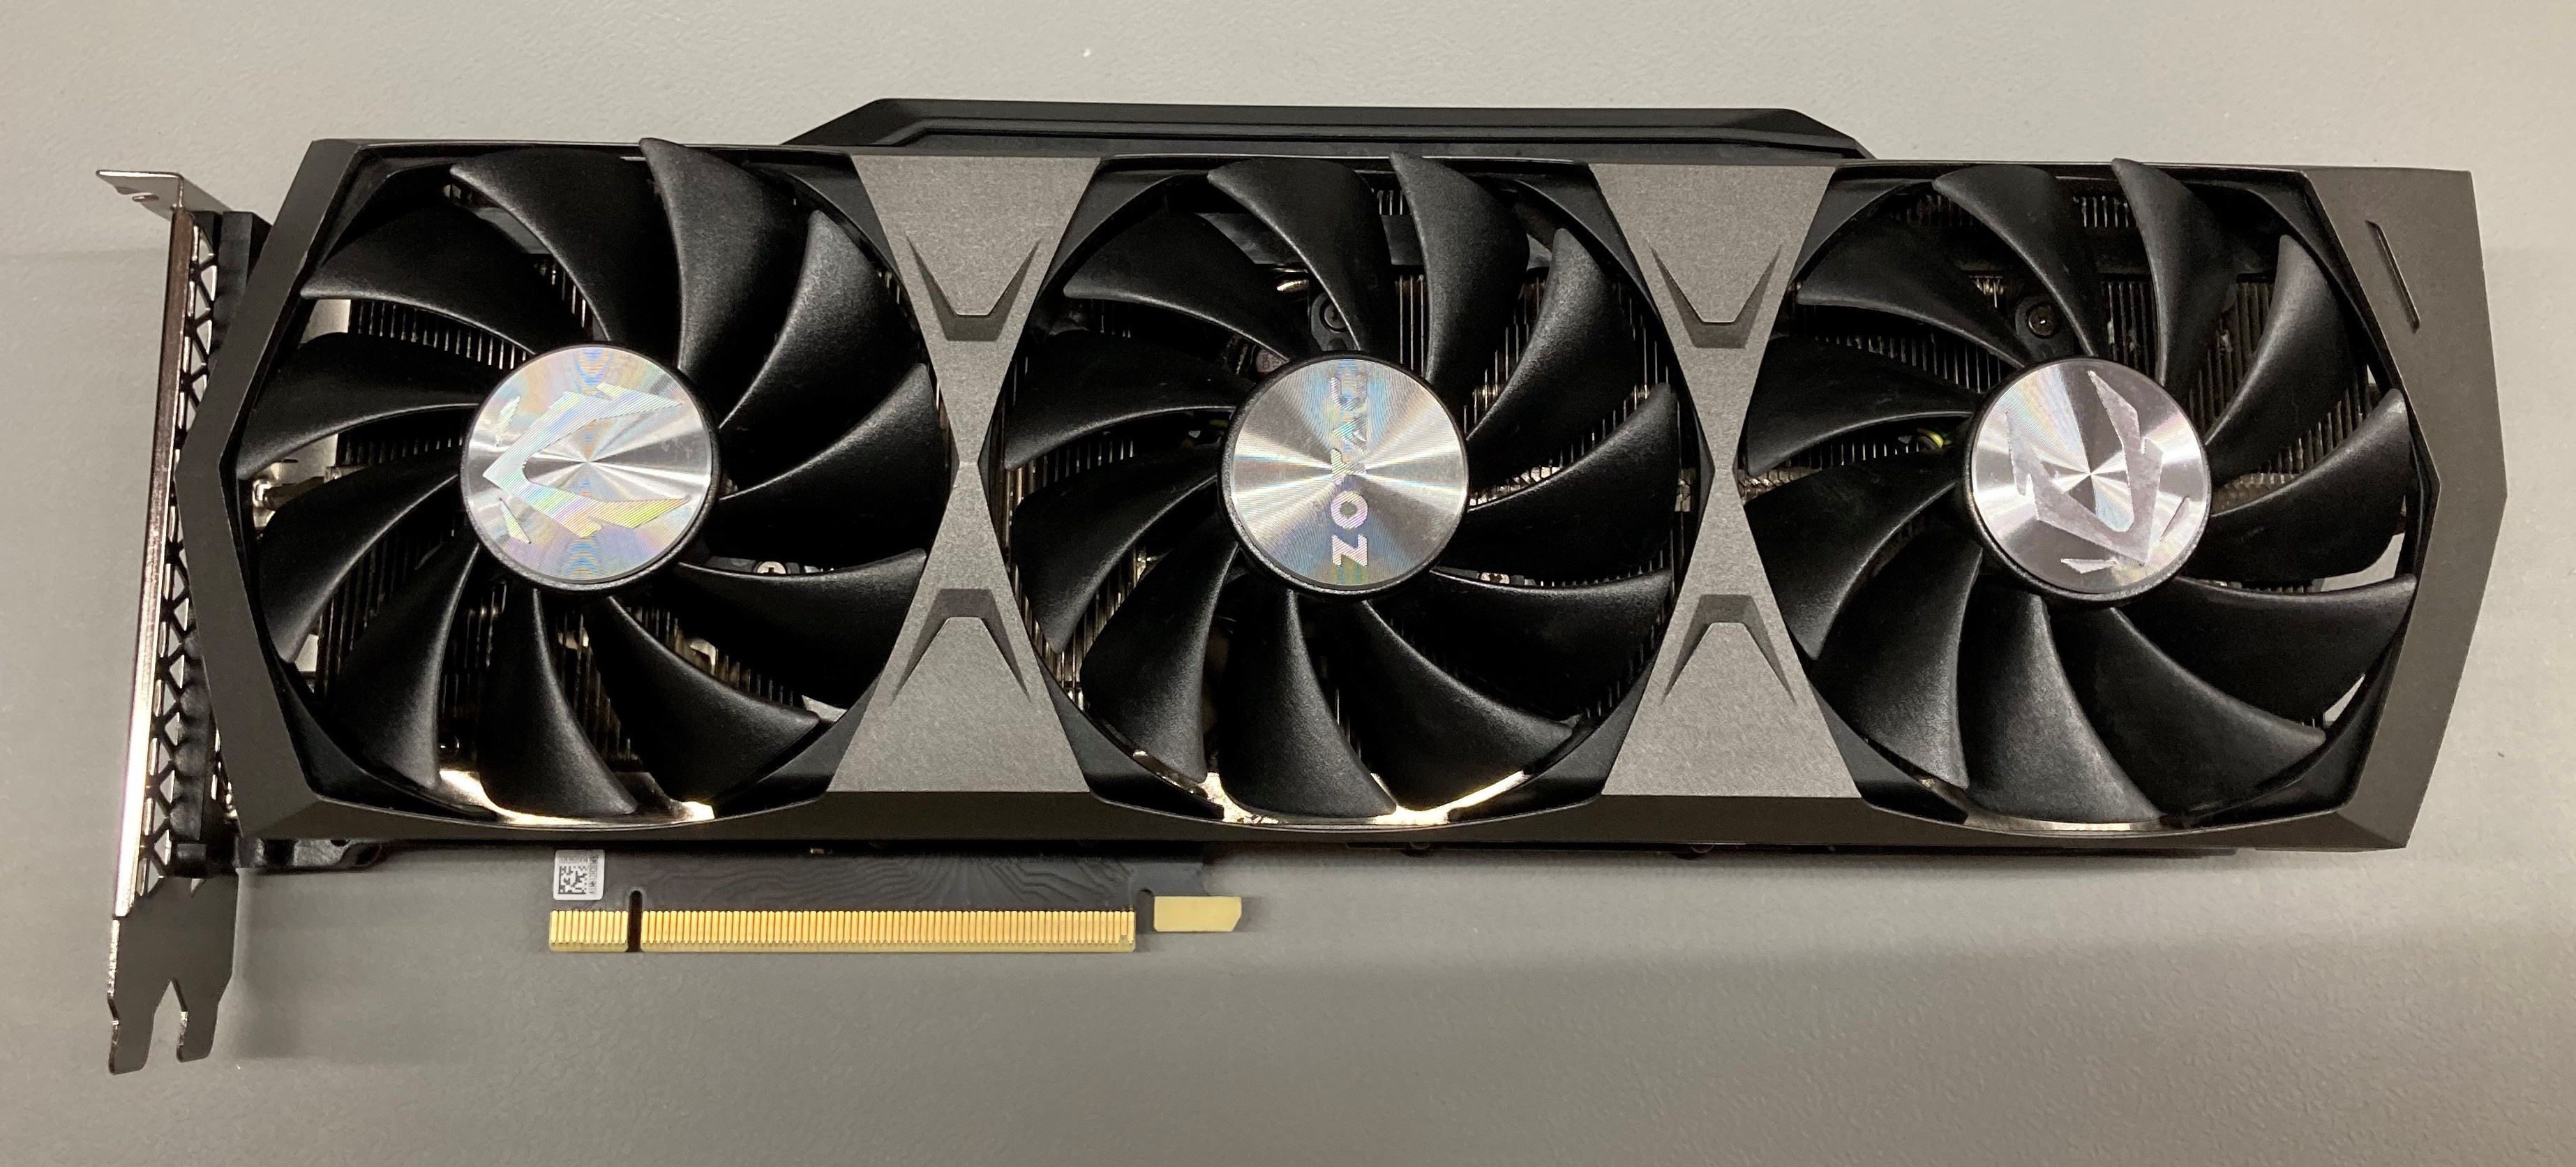
\includegraphics[width=10cm]{01_Ventilator-Zijde}
\centering
	\caption{GPU: Ventilatoren (Foto: Alex van Vianen)}
\label{fig:gpu:ventilator}
\end{figure}

Onder de ventilator treffen we de GPU en het video geheugen aan.

\begin{figure}[h]
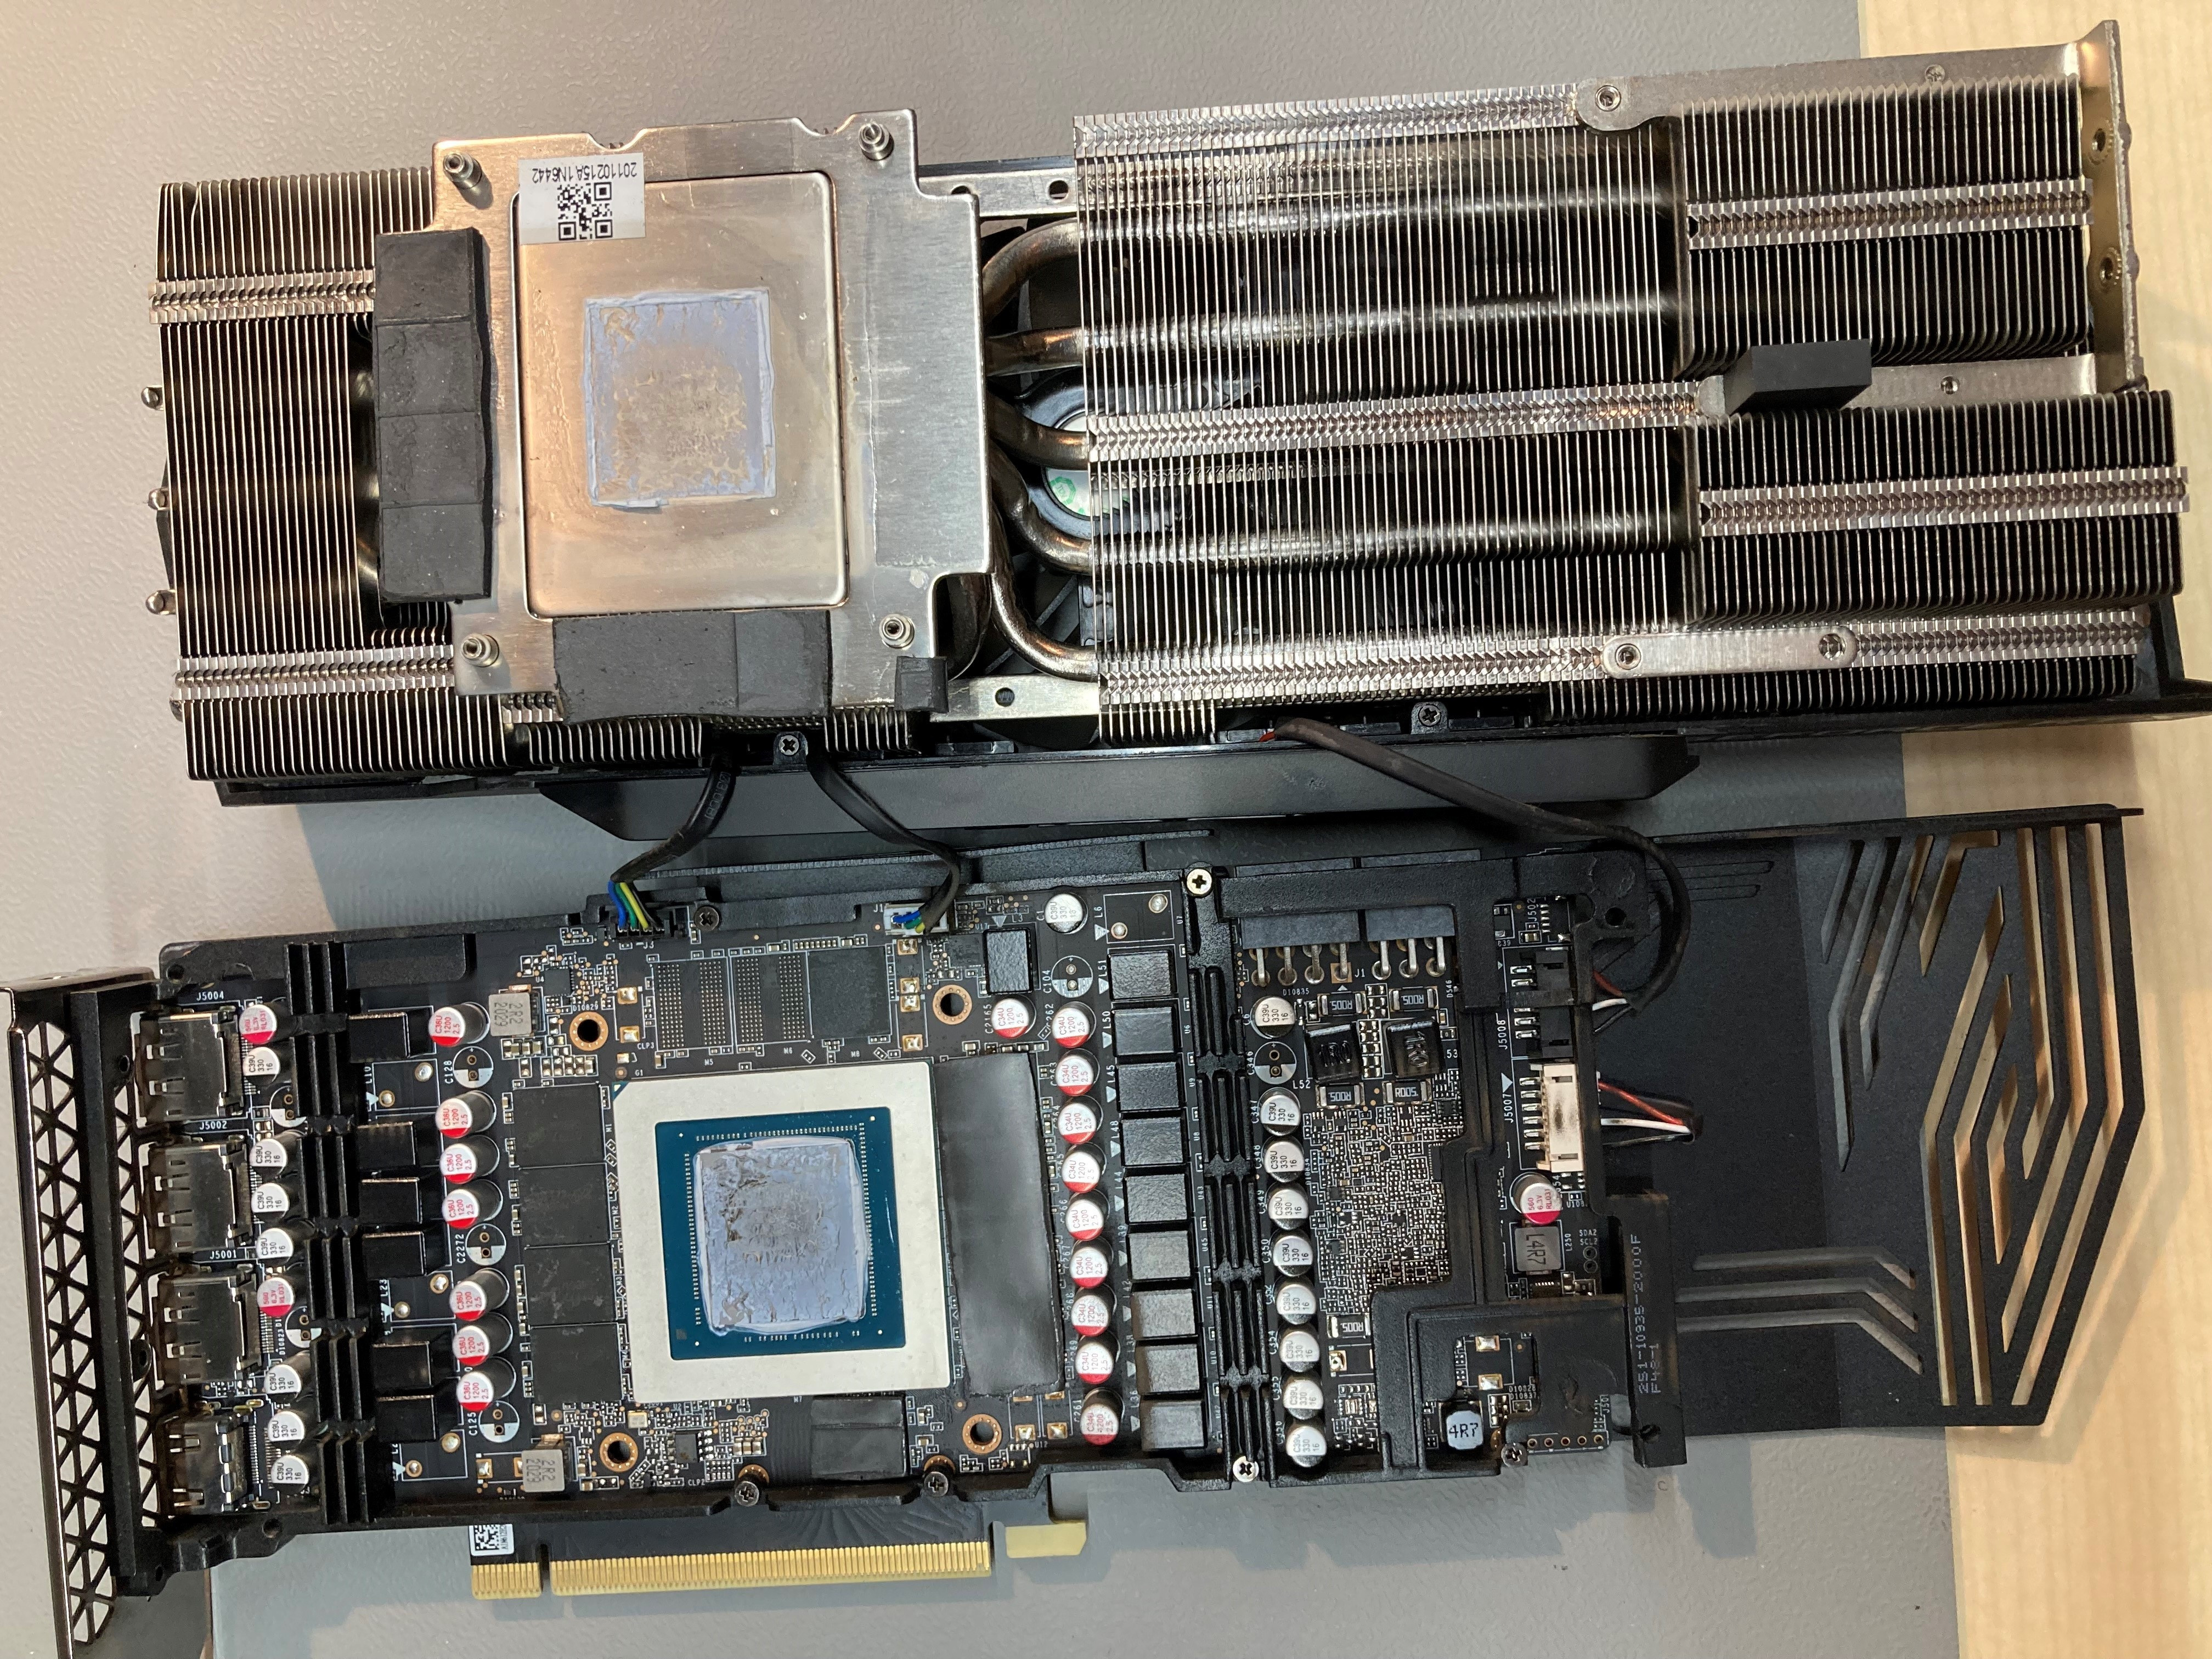
\includegraphics[width=10cm]{03_Opengewerkte_GPU}
\centering
	\caption{GPU: Ventilatoren verwijderd (Foto: Alex van Vianen)}
\label{fig:gpu:open}
\end{figure}

VRAM is een soort dynamic RAM. In het begin werd er gewone RAM gebruikt op de video-kaart zodat de grafische processor zijn eigen geheugen had. Het voordeel van eigen geheugen is dat de PCI-bus ontlast werd. Er waren minder lees en schrijf transacties over de PCI bus naar het main-memory van de PC. De GPU kon direct met zijn eigen geheugen praten.

Er zijn verschillende types VRAM:
\begin{description}
	\item [Multibank DRAM] VRAM opgedeeld in verschillende units waardoor de performance toeneemt
	\item [Synchronous Graphics RAM] 
	\item [Window VRAM] gebruikt in omgevingen met true-color en en hoge-resolutie. Heeft tot 25\% meer bandbreedte.
\end{description}

\begin{figure}[h]
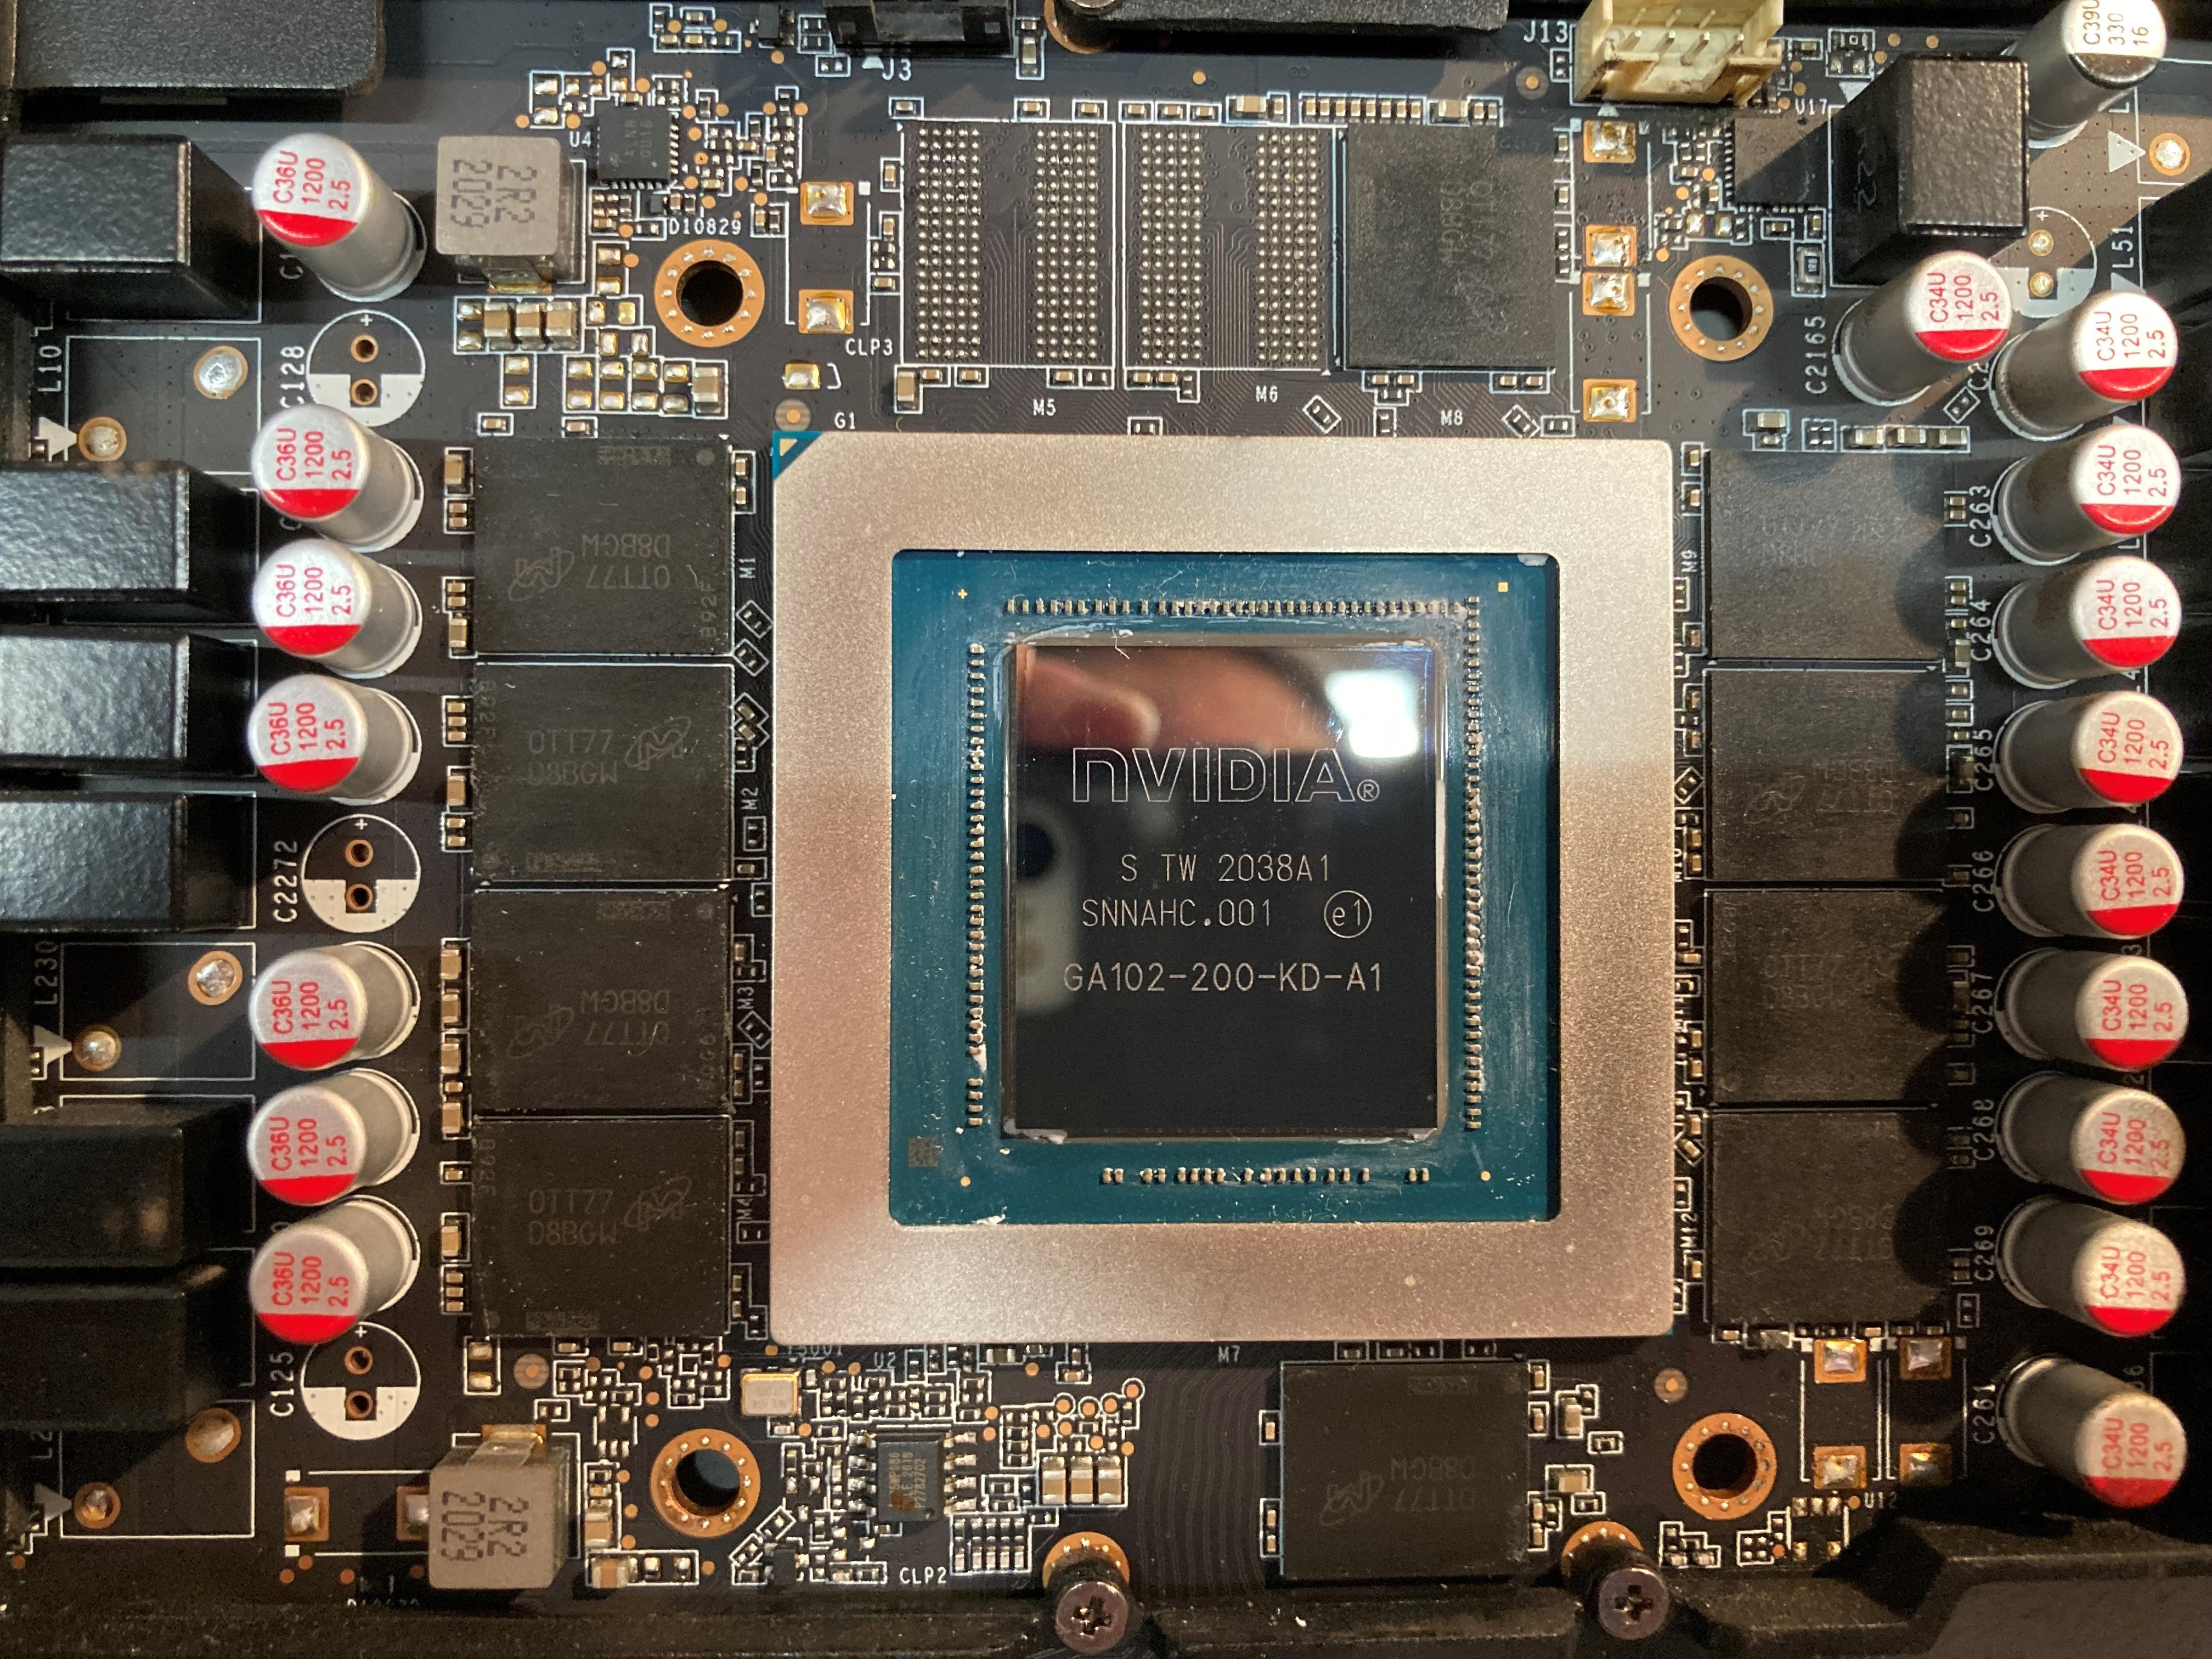
\includegraphics[width=10cm]{06_GPU_VRAM_Gereinigd}
\centering
	\caption{GPU en VRAM (Foto: Alex van Vianen)}
\label{fig:gpuvram}
\end{figure}

\begin{figure}[h]
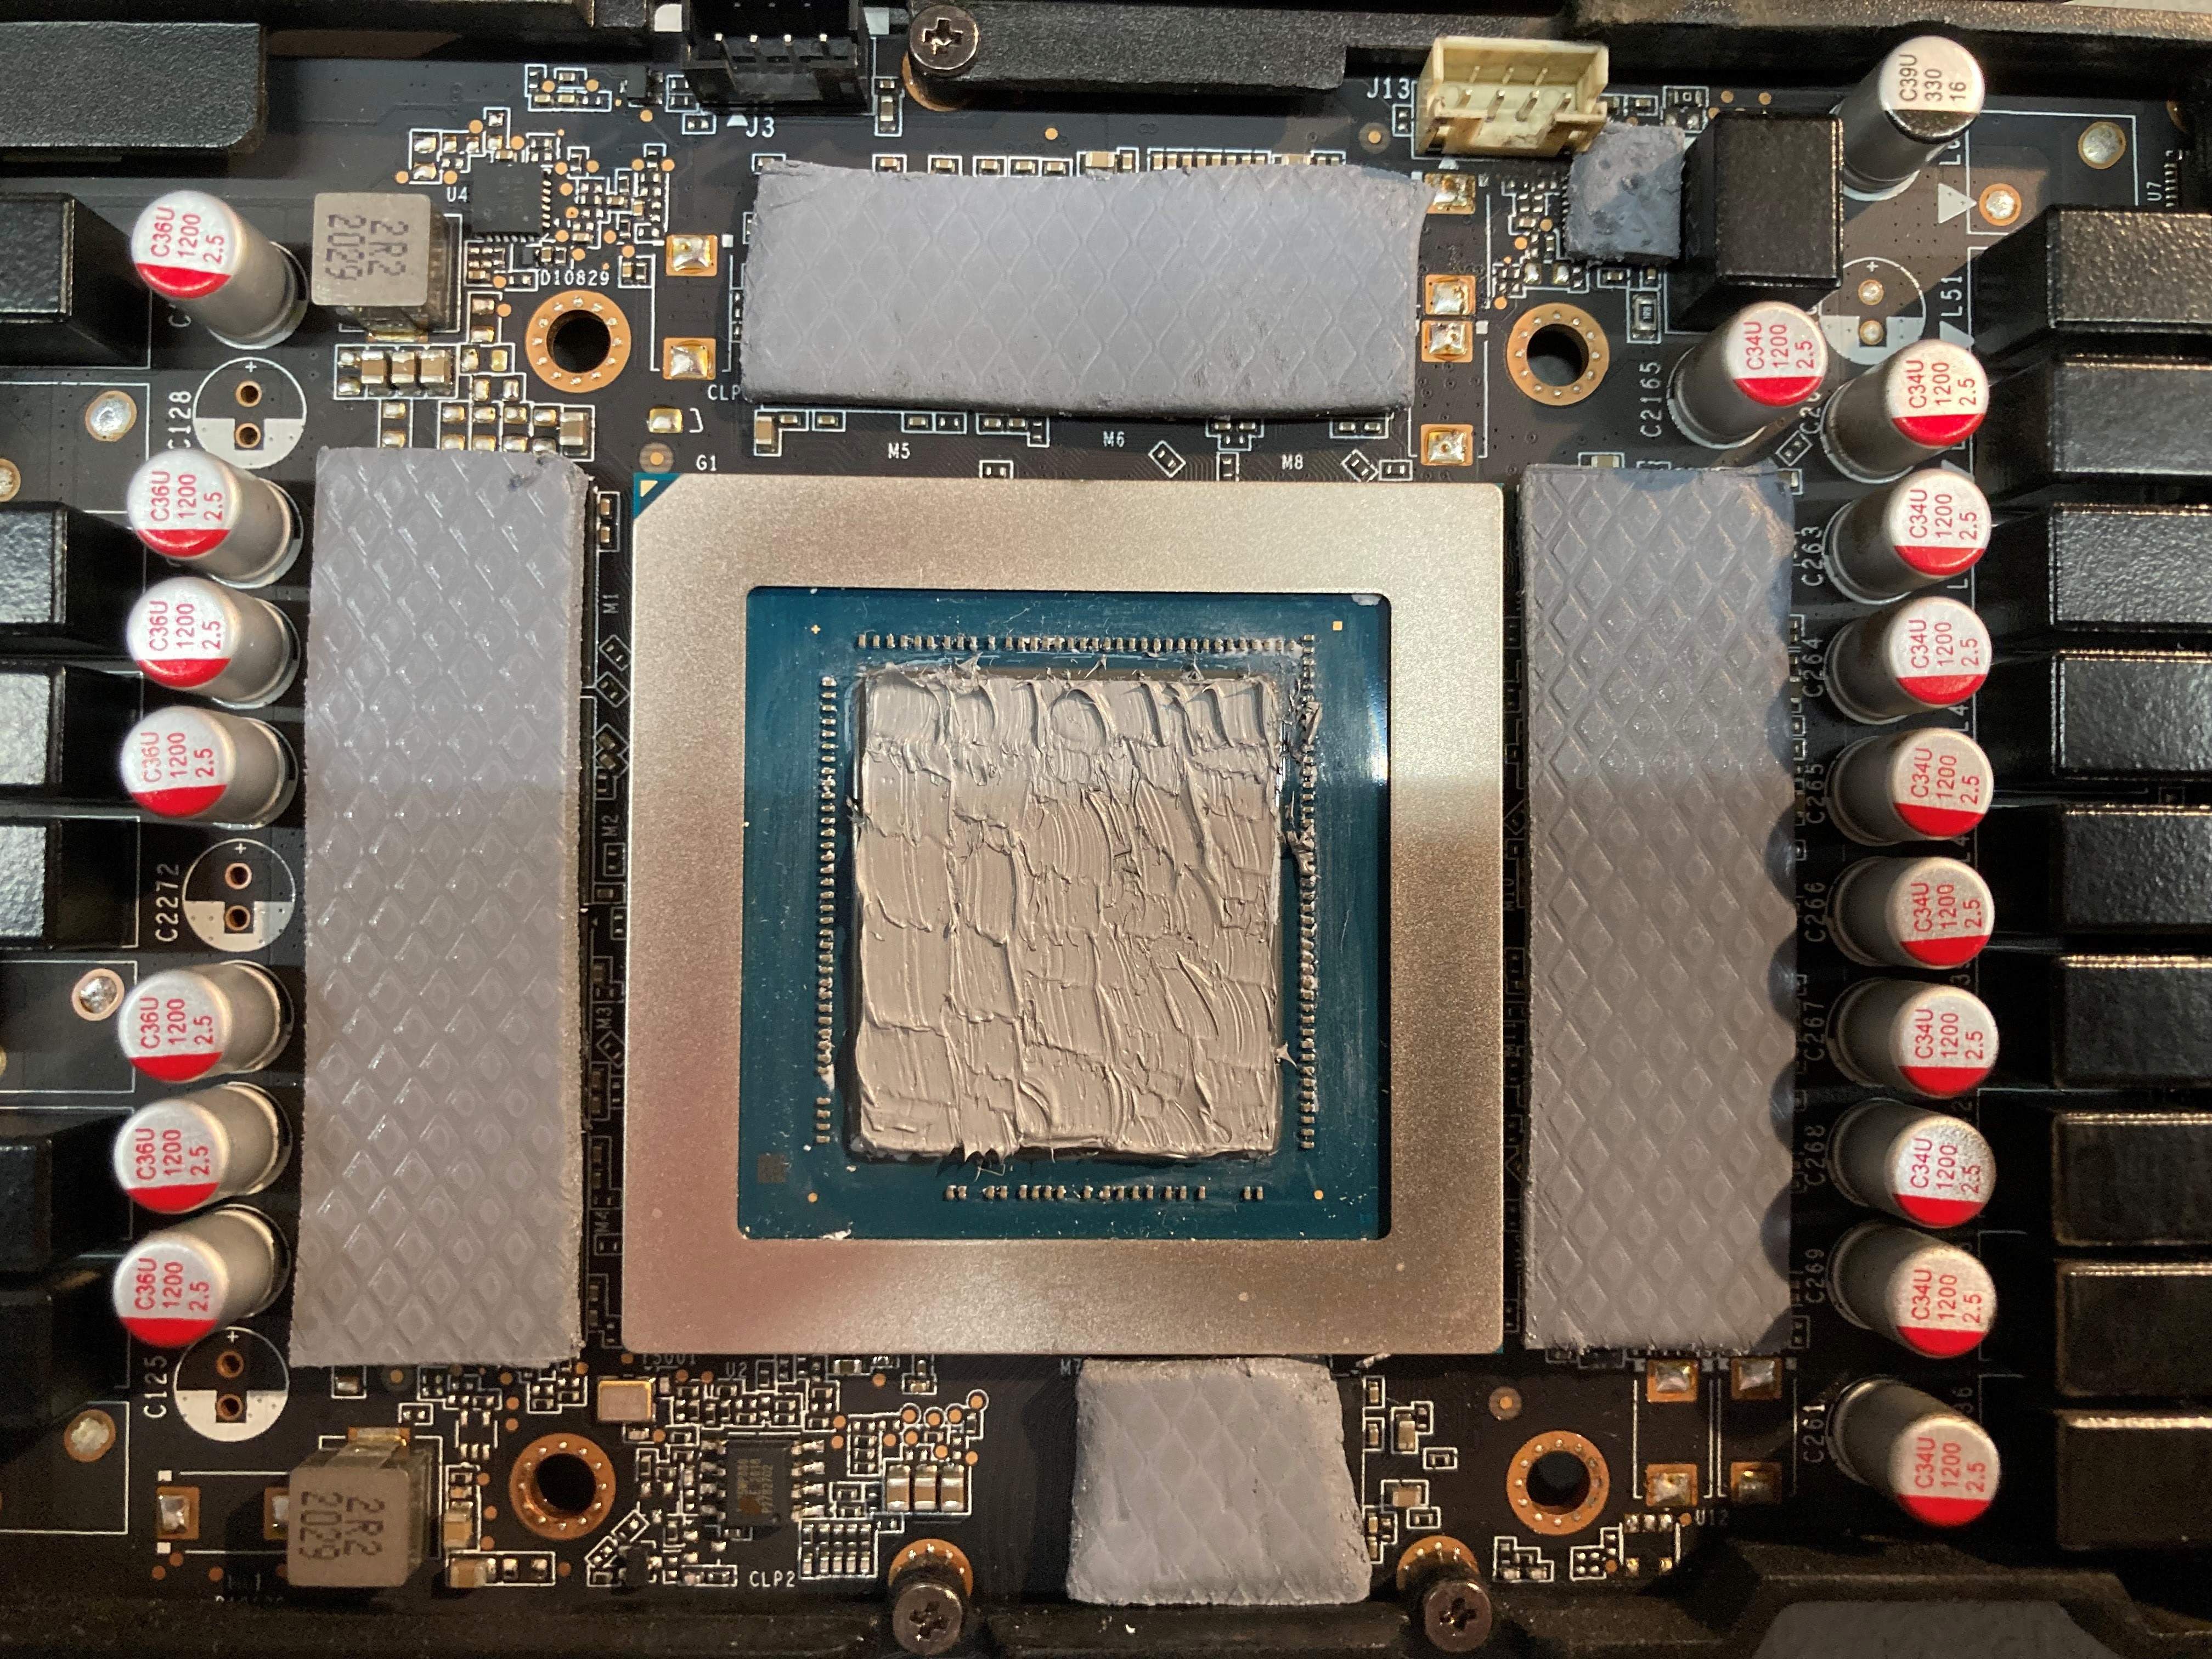
\includegraphics[width=10cm]{09_Nieuwe_Koelpasta_Aangebracht}
\centering
	\caption{GPU met thermalpads en koelpasta (Foto: Alex van Vianen)}
\label{fig:gputhermalpasta}
\end{figure}

